% v2-acmlarge-sample.tex, dated March 6 2012
% This is a sample file for ACM large trim journals
%
% Compilation using 'acmlarge.cls' - version 1.3, Aptara Inc.
% (c) 2011 Association for Computing Machinery (ACM)
%
% Questions/Suggestions/Feedback should be addressed to => "acmtexsupport@aptaracorp.com".
% Users can also go through the FAQs available on the journal's submission webpage.
%
% Steps to compile: latex, bibtex, latex latex
%
\documentclass[prodmode,acmtap]{acmlarge}

% Metadata Information
\acmVolume{4}
\acmNumber{3}
\acmArticle{} % value doesn't matter
\articleSeq{34} % minimum value to make the right margin black box disappear
\acmYear{1982}
\acmMonth{7}

% Package to generate and customize Algorithm as per ACM style
\usepackage{multirow}
\usepackage{rotating}
\usepackage[ruled]{algorithm2e}
\SetAlFnt{\algofont}
\SetAlCapFnt{\algofont}
\SetAlCapNameFnt{\algofont}
\SetAlCapHSkip{0pt}
\IncMargin{-\parindent}
\renewcommand{\algorithmcfname}{ALGORITHM}

\newcommand\prob{Problem of Heads of a Fighting Force from Long Ago}
% Page heads
\markboth{L. Lamport, R. Shostak, and M. Pease}{The \prob}

% Title portion
\title{The \prob}
\author{LESLIE LAMPORT, ROBERT SHOSTAK, and MARSHALL PEASE \\
SRI In Many Lands
}
% NOTE! Affiliations placed here should be for the institution where the
%       BULK of the research was done. If the author has gone to a new
%       institution, before publication, the (above) affiliation should NOT be changed.
%       The authors 'current' address may be given in the "Author's addresses:" block (below).
%       So for example, Mr. Fogarty, the bulk of the research was done at UIUC, and he is
%       currently affiliated with NASA.

\begin{abstract}
Sometimes, in a group of computers, there will be a broken part that will tell
confusing facts to the rest of the computers in the group. If we want to be
able to trust the entire group, it must be able to ignore these confusing facts
when deciding what to do. We can talk about this situation by playing
make-believe about the heads of a fighting force from long ago, who are waiting
with their people around a bad-guy city. The people must agree upon a shared
fighting plan, but can only talk to each other by sending a person who carries
a letter with orders written on it. However, one or more of the heads may be
bad guys who will try to confuse the others. The problem is to find a way for
the good guys to talk to each other, without knowing who the bad guys are, to
make sure they can agree on what to do anyway. We will show that, if the good
guys use only word-of-mouth, this problem is possible if and only if more than
two-thirds of the heads are good guys. This means that a single bad guy could
confuse two good guys. If the good guys use signed written letters, which means
a bad guy couldn't pretend their letter came from someone else, the problem is
possible for any number of heads and possible bad guys.
% Finally we will talk about ways to use the plans that are answers to this problem in different situations in the real world.
\end{abstract}

% Words about what this paper is about:
\category{C.2.4.}{Computer-Talking Groups}{Groups of many computers}[groups of brains of computers]
\category{D.4.4}{Computer Brains}{Managing Talking}[talking in groups]
\category{D.4.5}{Computer Brains}{Being Trusted}[accepting faults]

%Big Picture Words
\terms{Plans, Being Trusted}

%More Key Words and Groups of Words
\keywords{Friends agreeing with themselves}

%\acmformat{Daniel Pineo, Colin Ware, and Sean Fogarty. 2009. Neural Modeling of Flow Rendering Effectiveness.}
% At a minimum you need to supply the author names, year and a title.
% IMPORTANT:
% Full first names whenever they are known, surname last, followed by a period.
% In the case of two authors, 'and' is placed between them.
% In the case of three or more authors, the serial comma is used, that is, all author names
% except the last one but including the penultimate author's name are followed by a comma,
% and then 'and' is placed before the final author's name.
% If only first and middle initials are known, then each initial
% is followed by a period and they are separated by a space.
% The remaining information (journal title, volume, article number, date, etc.) is 'auto-generated'.

\begin{document}
\setcounter{page}{382}

\begin{bottomstuff}
This work was helped in part by the People Who Go To Space under plan NAS1-15428 Change 3, the Group for Being Safe Against Flying Fire Guns under plan DASG60-78-C-0046, and the Fighting Force Work Office under plan DAAG29-79-C-0102.

Where the people who wrote this live: Computer Study Work Place, SRI In Many Parts of the World, 333 Flying Animal's Wood Street, Park with a Person's Name, CA 94025.
\end{bottomstuff}


\maketitle

% Head 1
\section{Opening Words}

If you have a group of computers that you want to be able to trust, it must be able to live even if one of its parts breaks.
A broken part may act in a way that people often don't think about -- that is, sending confusing facts to different parts of the computer-group.
We will talk about this kind of breaking-problem, using make-believe, as the \prob.
%We spend the biggest part of the paper to talking about this make-believe problem and finish by showing how our answers can be used in building a group of computers that can be trusted.

We imagine that several parts of the fighting force from long ago are waiting outside a bad-guy city, each group controlled by its own head person. The heads can talk with one another only by sending a person who carries a letter with the orders written on it. After watching the bad guys, they must decide upon a shared plan of attack. However, some of the heads may be bad guys, trying to stop the good guys heads from agreeing. The heads must have an plan to make sure that: \\
\\
A. All good guys decide upon the same plan of how to act. \\

The good guy heads will all do what the plan says they should, but the bad guy heads may do anything they wish. The plan must make sure that situation A happens no matter what the bad guys do.

\newcommand\fact{\ensuremath{\mathsf{fact}}}

The good guys should not only agree, but should agree upon a plan that makes sense. So, we also want to make sure that \\
\\
B. A small number of bad guy heads can't cause the good guy heads to take a bad plan. \\

It is hard to make clear what we mean in Situation B, since it needs you to say exactly what a bad plan is or isn't, and we do not attempt to do so.
Instead, we consider how the heads reach a way to agree.
Each head watches the bad-guy city and tells what he or she sees to the others.
Let $\fact(i)$ be the facts told by the head with number $i$.
Each head uses some way to put together the facts $\fact(1) \dots \fact(n)$ into a single plan of what to do, where $n$ is the number of heads.
We can make Situation A happen by having all heads use the same way for putting together the facts, and make Situation B happen by using a way that can be trusted.
Think about this case: if the only thing to agree on is whether to attack or run away, then $\fact(i)$ can be Head $i$'s thought of which way is best, and the real plan can come from which way has more heads that want to do it.
A small number of bad guys can change the way only if there were almost the same number of good guys who wanted to do each way, in which case not either way could be called bad.

While this approach may not be the only way to make situations A and B happen, it is the only one we know of.
It needs a way for the heads to tell their facts $\fact(i)$ to one another. The most clear way is for the head number $i$ to send $\fact(i)$ by a person who carries a letter to each other head. However, this does not work, because making situation A happen needs every good guy head to read the same facts $\fact(1) \dots \fact(n)$, and a bad guy head may send different facts to different heads. For situation A to happen, the following must be true: \\
\\
1. Every good guy head must hear the same facts $\fact(1) \dots \fact(n)$. \\

Situation 1 means that a head can't in all cases use a fact of $\fact(i)$ read straight from the head number $i$, since a bad guy head number $i$ may send different facts to different heads.
This means that without care, in meeting situation 1 we might make it possible for the heads to use a fact for $\fact(i)$ different from the one sent by head number $i$--even though that head is good.
We must not allow this to happen if situation B is to be met. Think about this case: we can't allow a few bad guys to cause the good guys to act as if the facts were ``run away'' , \dots, ``run away'' if every good guy said ``attack''.
So, we need the following thing for each $i$: \\
\\
2. If head number $i$ is good, then the fact that he or she sends must be used by every good guy head as the fact for $\fact(i)$. \\

We can say situation 1 another way by saying that for every $i$ (whether or not the head number $i$ is a good guy), \\
\\
1'. Any two good guy heads use the same meaning of $\fact(i)$. \\

Situations 1' and 2 both use just the single fact that was sent by head number $i$.
Because of this, we can think about the smaller problem of how a single head sends their fact to the others. We'll talk about this by talking about a controlling head sending a letter to her friends, causing the following problem. \\

{\em The \prob.} A controlling head must send an order to her n-1 friends such that \\
FA1. All good-guy friends listen to the same order. \\
FA2. If the controlling head is a good guy, then every good guy friend listens to the order she sends. \\

These situations, FA1 and FA2, are called the {\em friends agreeing} situations. Note that if the controlling head is a good guy, then FA1 follows from FA2. However, the controlling head need not be good.

\newcommand\shortprob{Fighting Force Heads Problem}
To fix our first problem, head number i sends their fact of $\fact(i)$ by using an answer to the \shortprob~to send the order ``use $\fact(i)$ as my fact'', with the other heads acting as the helping friends.

\section{Showing What Isn't Possible}

The Problem of Heads of a Fighting Force from Long Ago seems simple, but it is actually not. It is hard because of the surprising fact that if the heads can send only talk to each other out loud, then any plan can only work if more than two-thirds of the heads are good guys. Now, when we say ``talking out loud'', we mean that the words are completely under the control of the person saying them, so a bad guy could say anything he or she wanted to, even ``Your good-guy friend said to do such-and-such!''
This sort of speaking is the same as how computers usually speak to one another. In Part~\ref{sec:4}, we consider signed, written letters, for which this is not true.

We now show that with spoken words, no plan for three people can handle a single bad guy.
To keep things simple, we consider the case in which the only things to do are ``attack'' or ``run away''.
Let us first think about the situation pictured in Figure~\ref{fig:1} in which the controlling head is a good guy, and sends an ``attack'' order, but the second friend is a bad guy and tells the first friend that he heard a ``run away'' order. For FA2 to happen, the first friend must listen to the order to attack.

Now consider another situation, shown in Figure~\ref{fig:2}, in which the controlling head is actually a bad guy, and sends an ``attack'' order to the first friend and a ``run away'' order to the second friend. The first friend does not know who the bad guy is, and she can't tell what the controlling head actually said to the second head. So, the situations in these two pictures appear exactly the same to the first friend. If the bad guy lies all the time, then there is no way for the first friend to know which situation is happening, so she must listen to the ``attack'' order in both of them. So, any time the first friend hears an ``attack'' order from the controlling head, she must listen to it.

\begin{figure}[h]
	\begin{center}
		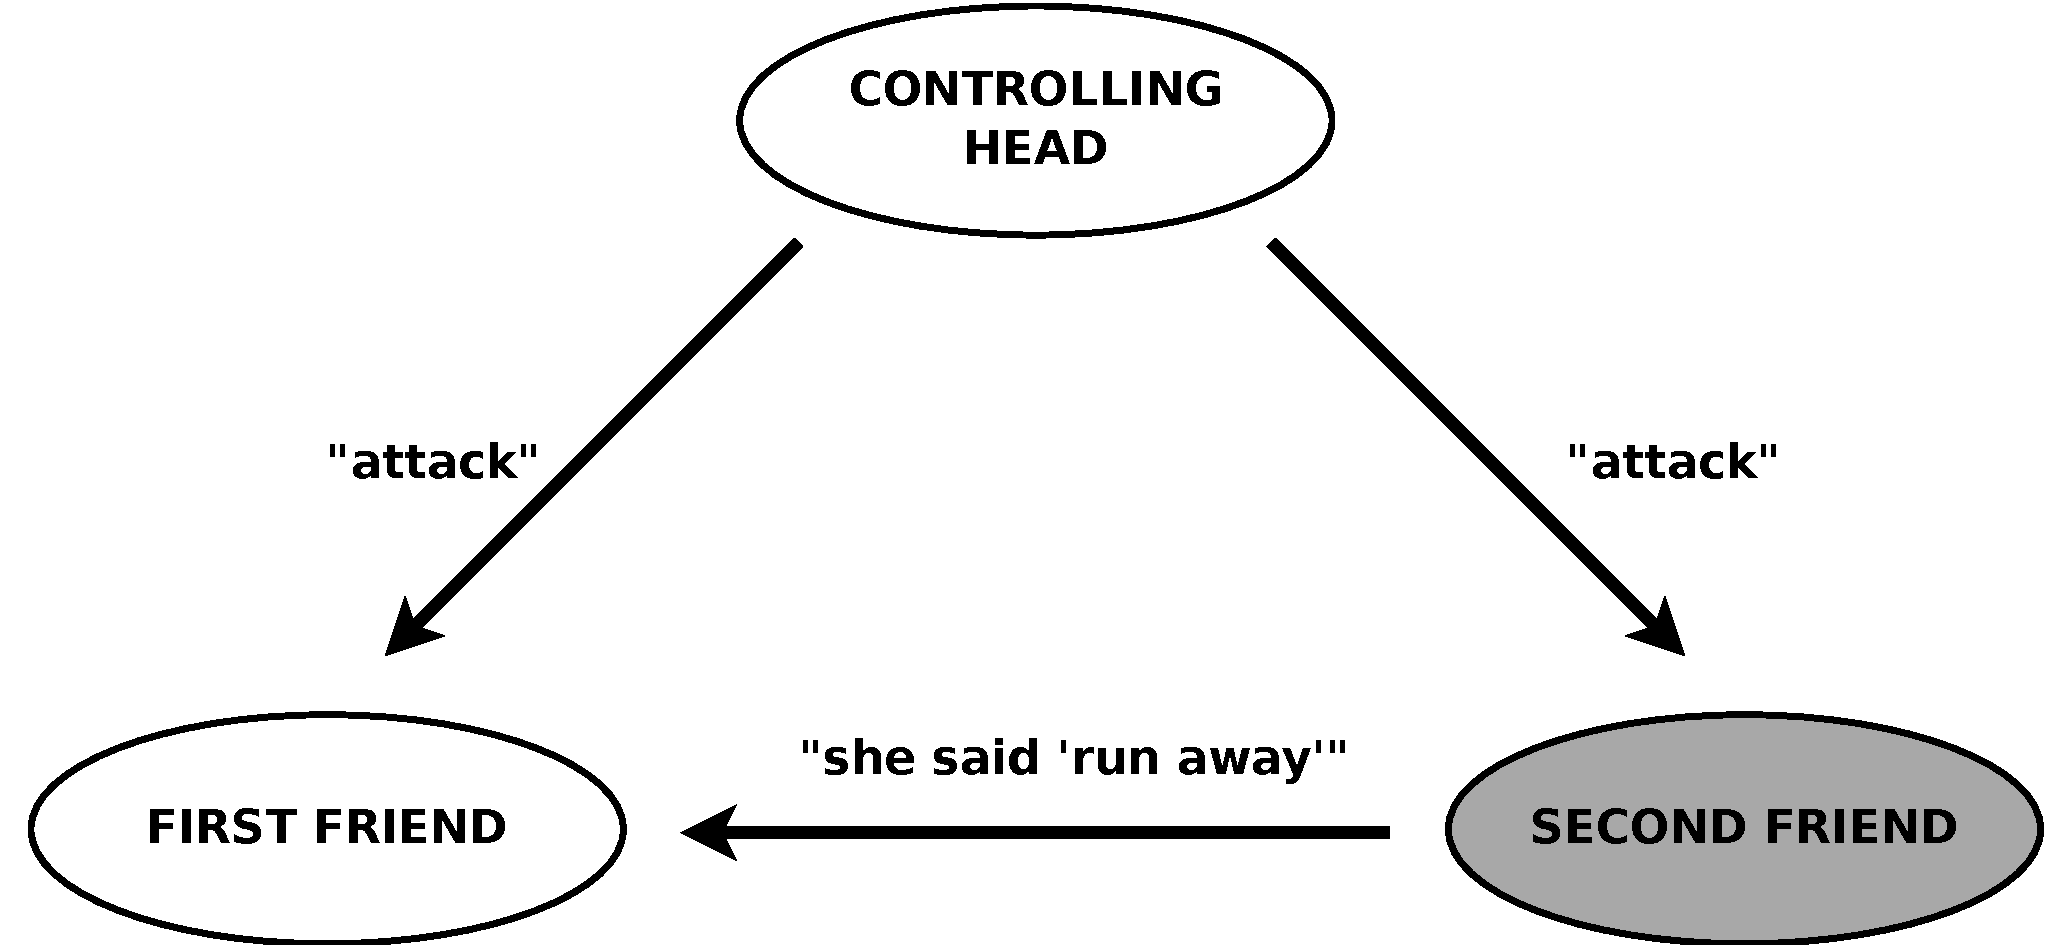
\includegraphics[width=0.7\textwidth]{fig1.pdf}
	\end{center}
	\caption{The second friend is a bad guy.}
	\label{fig:1}
\end{figure}
\begin{figure}[h]
	\begin{center}
		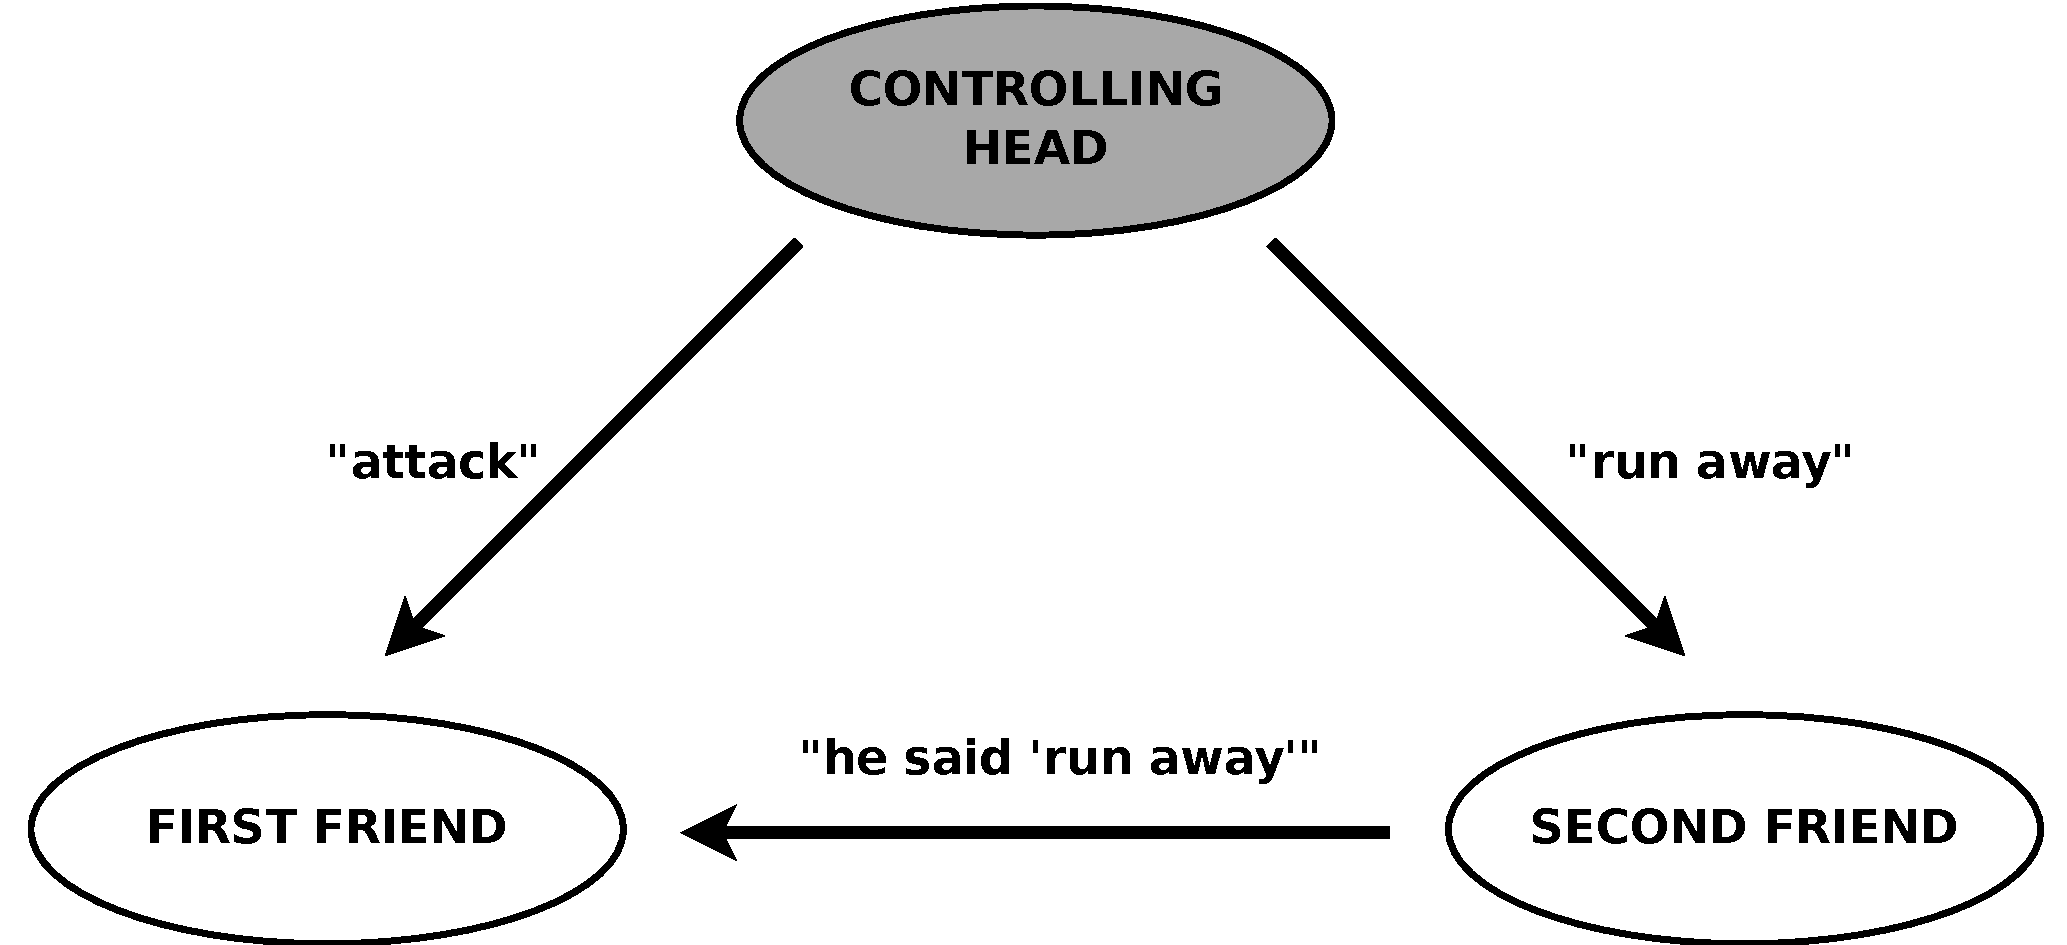
\includegraphics[width=0.75\textwidth]{fig2.pdf}
	\end{center}
	\caption{The controlling head is a bad guy.}
	\label{fig:2}
\end{figure}

However, in the same way we could show that if the second friend hears a ``run away'' order from the controlling head then he must listen to it even if the first friend tells him that the head said ``attack''. Because of this, in Figure 2, the second friend must listen to the ``run away'' order while the first friend listens to the ``attack'' order, which means situation FA1 doesn't happen. So, there is no way for three people to agree if one of them is a bad guy.

This way of thinking about it may appear right, but you should think hard before believing such hand-waving reasoning. Although what we said is right after all, we have seen other ``ways of thinking about it'' that are totally wrong.
We know of no area in the study of computers or the study of numbers in which hand-waving reasoning could more easily lead to wrong answers than in the study of this type of problem. For a stronger way of thinking about why this isn't possible, you should read [3].
Using this answer, we can show that no plan can work for a given number of heads if one third of them are bad guys.
% Omitted: Albanian generals contradiction proof.

You might think that it's so hard to fix the \shortprob~because the heads need to agree with each other completely. Actually, this is not the case, and only-sort-of agreeing with each other is just as hard. Suppose that instead of trying to agree on a complete plan to attack, the heads must agree only upon a set of times, during which the attack should happen. We will say the controlling head needs to order the time of the attack, and the following two situations need to happen: \\
\\
FA1'. All good guys attack within 10 minutes of one another. \\
FA2'. If the controlling head is a good guy, then every other good guy attacks within 10 minutes of the time given in the controlling head's order. \\
\\
(We are supposing that the orders are given and thought about the day before the attack and that the time at which an order is heard doesn't matter--only the attack time given in the order matters.)

Like the \prob, there is no answer to this problem except when more than two-thirds of the heads are good guys. We make sure this is true by first showing that if there were an answer for three people that were okay with one bad guy, then we could answer the first problem, which we already showed was not possible. Suppose the controlling head wishes to send an ``attack'' or ``run away'' order. We'll say that she can show she wants to attack by ordering an attack time of 1:00, or he could show he wants to run away by ordering an attack time of 2:00.
 Each of her friends, that is, the other heads, will listen to her order in the following way.

\begin{enumerate}
	\item After hearing the attack time, a head does one of the following:
	\begin{enumerate}
		\item If the time is 1:10 or earlier, then attack.
		\item If the time is 1:50 or later, then run away.
		\item Or else, continue to step (2).
	\end{enumerate}
	\item Ask the other not-controlling head what they did in step (1).
	\begin{enumerate}
		\item If they did either of the first two things, then do the same thing they did.
		\item Or else, run away.
	\end{enumerate}
\end{enumerate}

It follows from FA2' that if the controlling head is a good guy, then her good guy friends will hear the right order in step (1), so situation FA2 happens. Also, FA1 follows from FA2, so we only need to make sure of FA1 when we suppose the controlling head is a bad guy. Since there is at most one bad guy, this means that both of her friends are good guys.
It follows from FA1' that if one friend decides to attack in step (1), then the other can't decide to run away in step (1). So, either they will both do the same thing in step (1) or at least one of them will wait until step (2).
In this case, it is easy to see that they both decide to do the same thing, so FA1 happens. This means we just built a three-person answer for the first problem, which is not possible.
So, we can't have a plan for three people that makes FA1' and FA2' happen if one of them is a bad guy.

Notice how we had one of the heads pretend to be $m$ other heads at the same time. We can now do that again to make sure that no answer with three times $m$ (or fewer) people can ever be okay with $m$ bad guys.
The way of making sure that's true is like the one for the first problem, and is left for the person reading this paper to do on their own.

\section{An answer for when the heads use spoken words}

We showed above that for an answer to the \prob~using spoken words to be okay with with $m$ bad guys, there must be more than three times $m$ heads in total. We will now give an answer that works for more than three times $m$ heads. However, we first want to make clear exactly what we mean by ``spoken words''.
Each head is supposed to follow some plan that tells them to send some facts to the other heads, and we suppose that a good guy will actually follow the plan.
When we say ``spoken words'', we mean that we're supposing the following things about the way the heads talk to each other: \\
\\
A1. Every word that is said can be heard by the person who is meant to hear it. \\
A2. Any person who hears something knows who said it. \\
A3. If someone tried to say something, but their words went missing, you can know that that happened. \\

By supposing A1 and A2, we make sure a bad guy can't cause two other people to not be able to talk each other or to think they said things that they didn't.
By supposing A3, we make sure a bad guy can't make people not be able to decide something by not saying anything at all.

The answers that we give in this part of the paper and in the following one only work if each head is able to speak to each other head without needing anyone in between to help.
% Decide whether to write this part -- prob. not
We would talk about answers which do not need this to happen, but we are leaving that part out of our paper so the paper does not get too long.
% In the part of this paper number five, we talk about answers which do not need this to happen.

A bad-guy controlling-head may decide not to send any order. Since the other heads must decide to follow some order, they need something to do if no-one tells them to do anything. We'll say RUN AWAY will be this order.

We will show how to run a Spoken Words plan by which a controlling-head sends an order to the rest of the heads. We'll talk about this plan by a way of supposing that, as long as the plan works for some number of heads, it can also work for one more than that many heads. So if we can show that, then we know it works for all possible numbers of heads.

We show that the Spoken Words plan, with some number $m$, is an answer to the \prob~for more than three times $m$ many heads, as long as there are $m$ or fewer bad guys.\\

{\em The Spoken Words plan where $m$ is nothing at all (which means there are no bad guys):}\begin{enumerate}
	\item The controlling head says what she decided to do to every other head.
	\item Each other head does the thing they heard the controlling head say, or does RUN AWAY if they didn't hear anything.
\end{enumerate}

{\em The Spoken Words plan where $m$ is one more than some other number $j$:}\begin{enumerate}
	\item The controlling head says what she decided to do to every other head.
	\item For each number $i$, let $\fact_i$ be the fact that head number $i$ heard from the controlling head, or else be RUN AWAY if they hear nothing. Head number $i$ acts as the controlling-head in the Spoken Word plan for one fewer than $m$, to say $\fact_i$ to the other heads.
	\item For each number $i$, and each number $j$ not the same as $i$, let $\fact_j$ be the fact that head number $i$ heard from head number $j$ in step (2) (using the Spoken Word plan for one fewer than $m$), or else RUN AWAY if they heard nothing. Head number $i$ will do the thing that they heard most often, from all the $\fact_j$.
\end{enumerate}

To understand how this plan works, we consider the case where $m$ is one and there are four total heads. Figure
%\ref{fig:3}
3
shows what the second head hears when the controlling head says some fact $f$, and the third head is a bad guy.
The third head says some other fact $g$. In step 3, the second head then heard $f$ two times and $g$ once, so decides to do the right thing, which is $f$.

Next, we see what happens if the controlling head is a bad guy. Figure
%\ref{fig:4}
4
shows what the other heads hear if the controlling head says whatever she wants, which we'll say are $x$, $y$, and $z$, because they can all be different.
Each other head hears all three different orders, so they all decide to do the same thing in step (3), no matter if $x$, $y$, and $z$ are the same.

The bigger Spoken Word plan, where there are two or more bad guys, uses the smaller plan many different times. This means that for more than one bad guy, each head will have to talk to the other heads many different times. But there has to be a way for each head to tell which facts are which. You can make sure there is a way to do this by having each head, just before saying some fact $\fact_i$, also says the number $i$, in step (2).

To make sure the Spoken Words plan is right for any number of bad guys, we first make sure the following expression is true.

\newtheorem{mylemma}{Expression}
\begin{mylemma}
	\label{lemma:1}
	For any numbers $m$ and $k$, the Spoken Words plan makes situation FA2 happen if there are more than $2k+m$ heads and at most $k$ bad guys.
\end{mylemma}

{\sc Reason That is True.}
We can show the reason this is true by thinking about it in a way of supposing it is true for a given number then showing it must also be true for one more than that number. In this case the number we will pay attention to is $m$. FA2 only talks about what must happen if the
controlling head is a good guy. First, using A1, it is easy to see that the most simple plan (the Spoken Words plan for no bad guys at all), so the expression is true for the starting case.
We now suppose the expression is true for one fewer than some number $m$, and show it is true for $m$.

\pagebreak
\thispagestyle{empty}
\begin{sideways}
	\begin{tabular}{p{2in}p{9in}p{2in}}
	\\
	\multicolumn{2}{c}{
		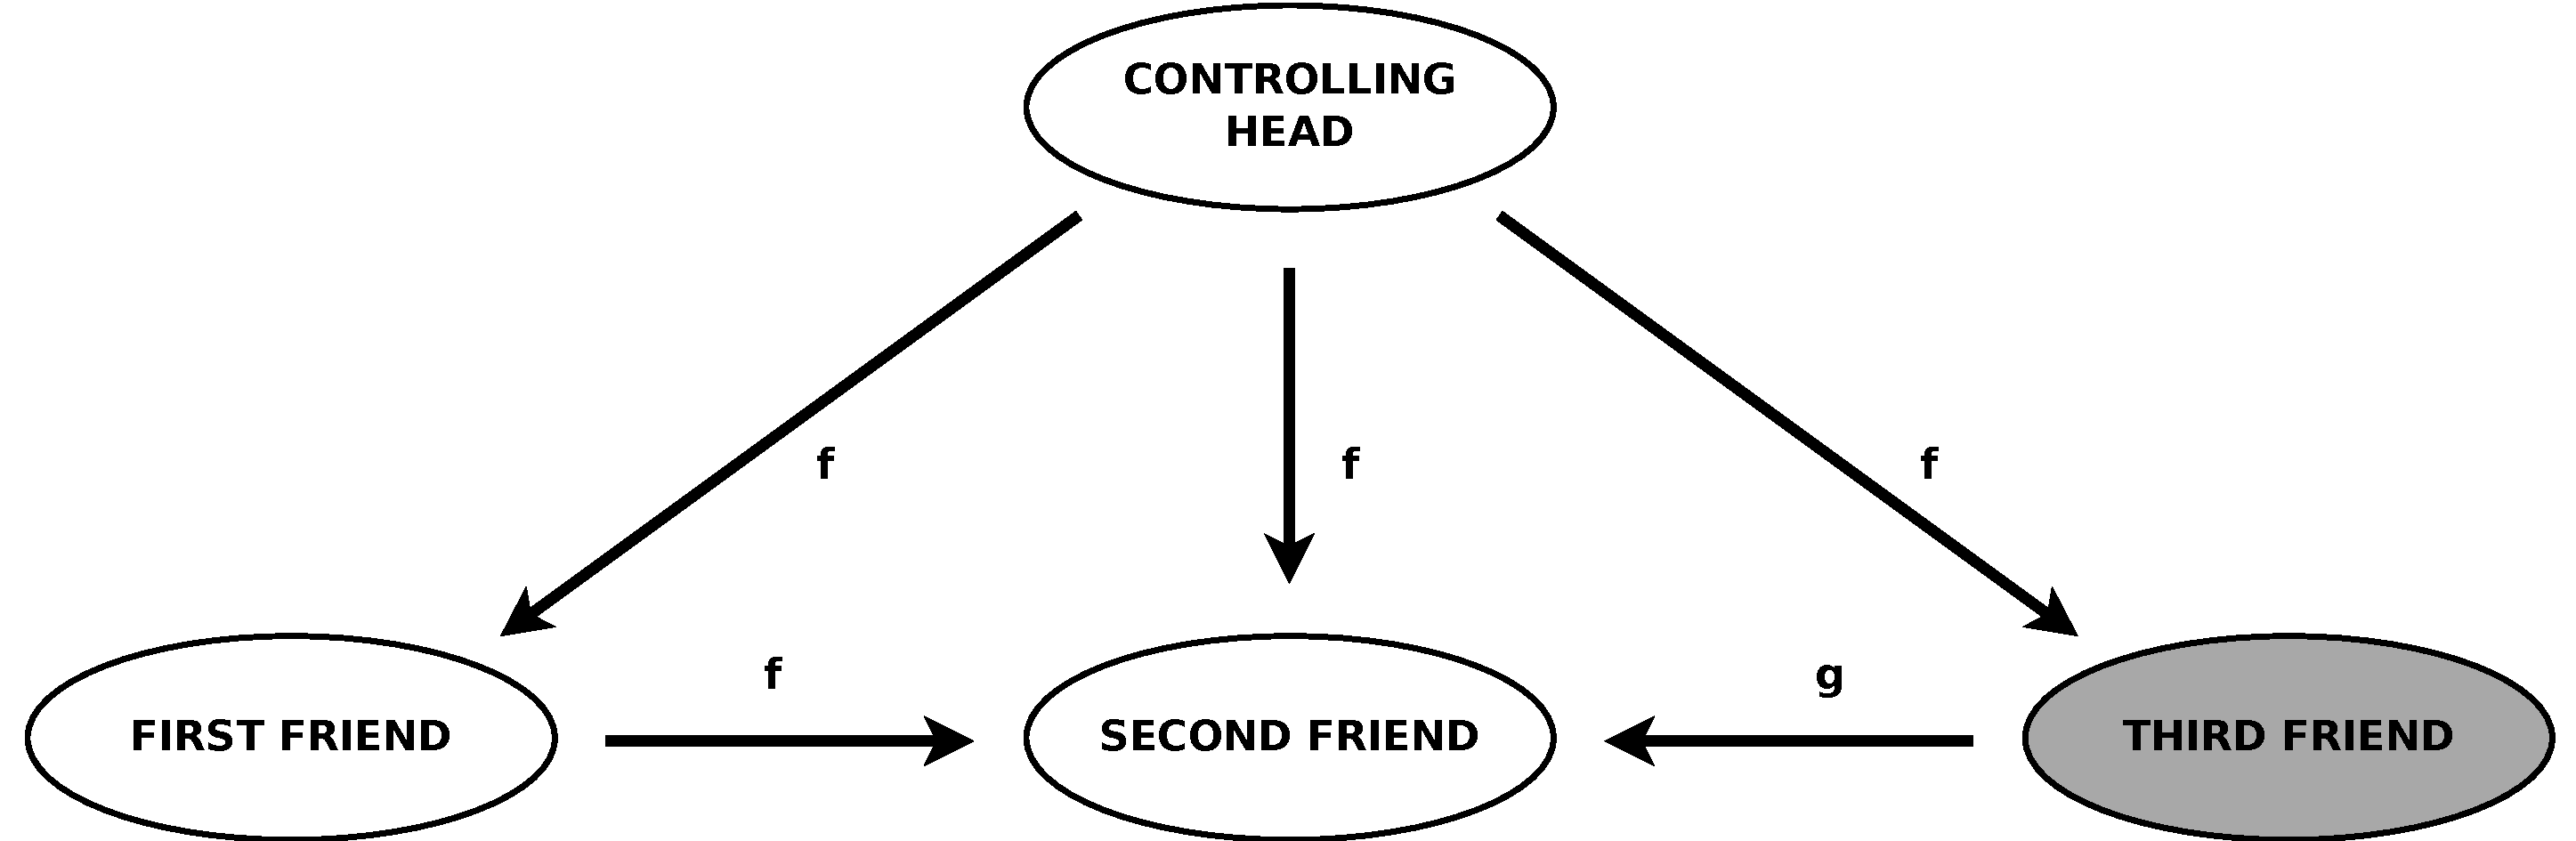
\includegraphics[width=0.95\textwidth]{fig3.pdf}
	}
	&
	\vspace{-8em}
	{\footnotesize Fig. 3. Spoken Words plan, where the third head is a bad guy.}
	\\
	\vspace{2em}
	\\
	\vspace{-10em}
	{\footnotesize Fig. 4. Spoken Words plan, where the controlling head is a bad guy.}
	&
	\multicolumn{2}{c}{
		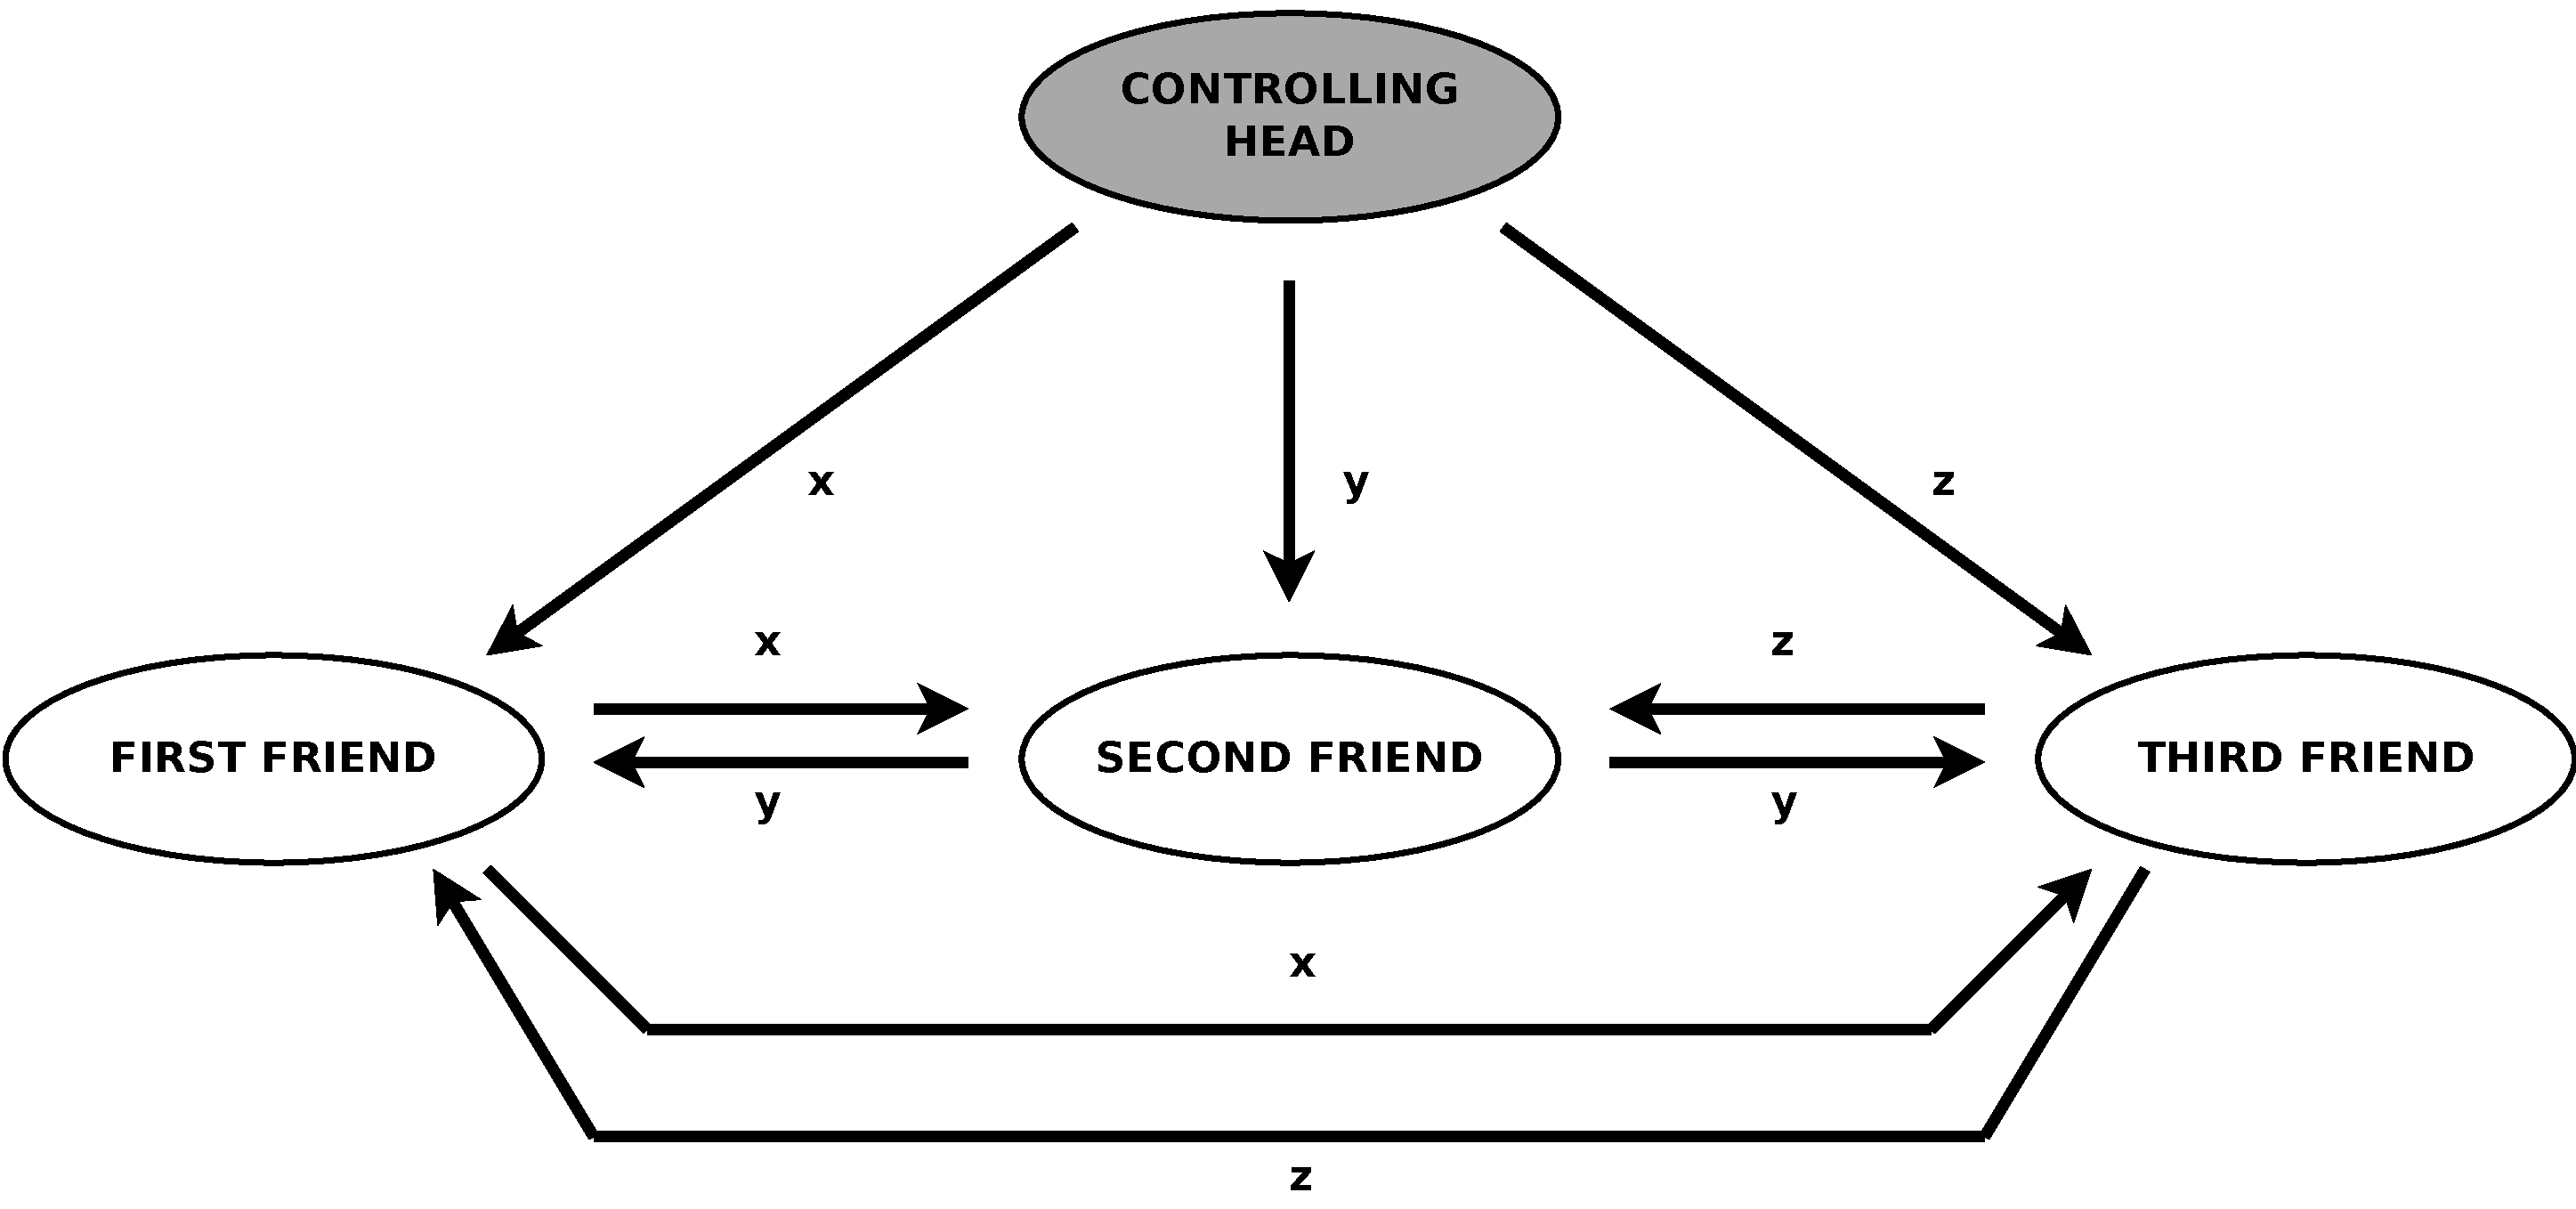
\includegraphics[width=0.95\textwidth]{fig4.pdf}
	}
	\end{tabular}
\end{sideways}
\pagebreak
\setcounter{figure}{4}

%\begin{figure}[h]
%	%\begin{sideways}\begin{minipage}{\textwidth}
%	\begin{center}
%		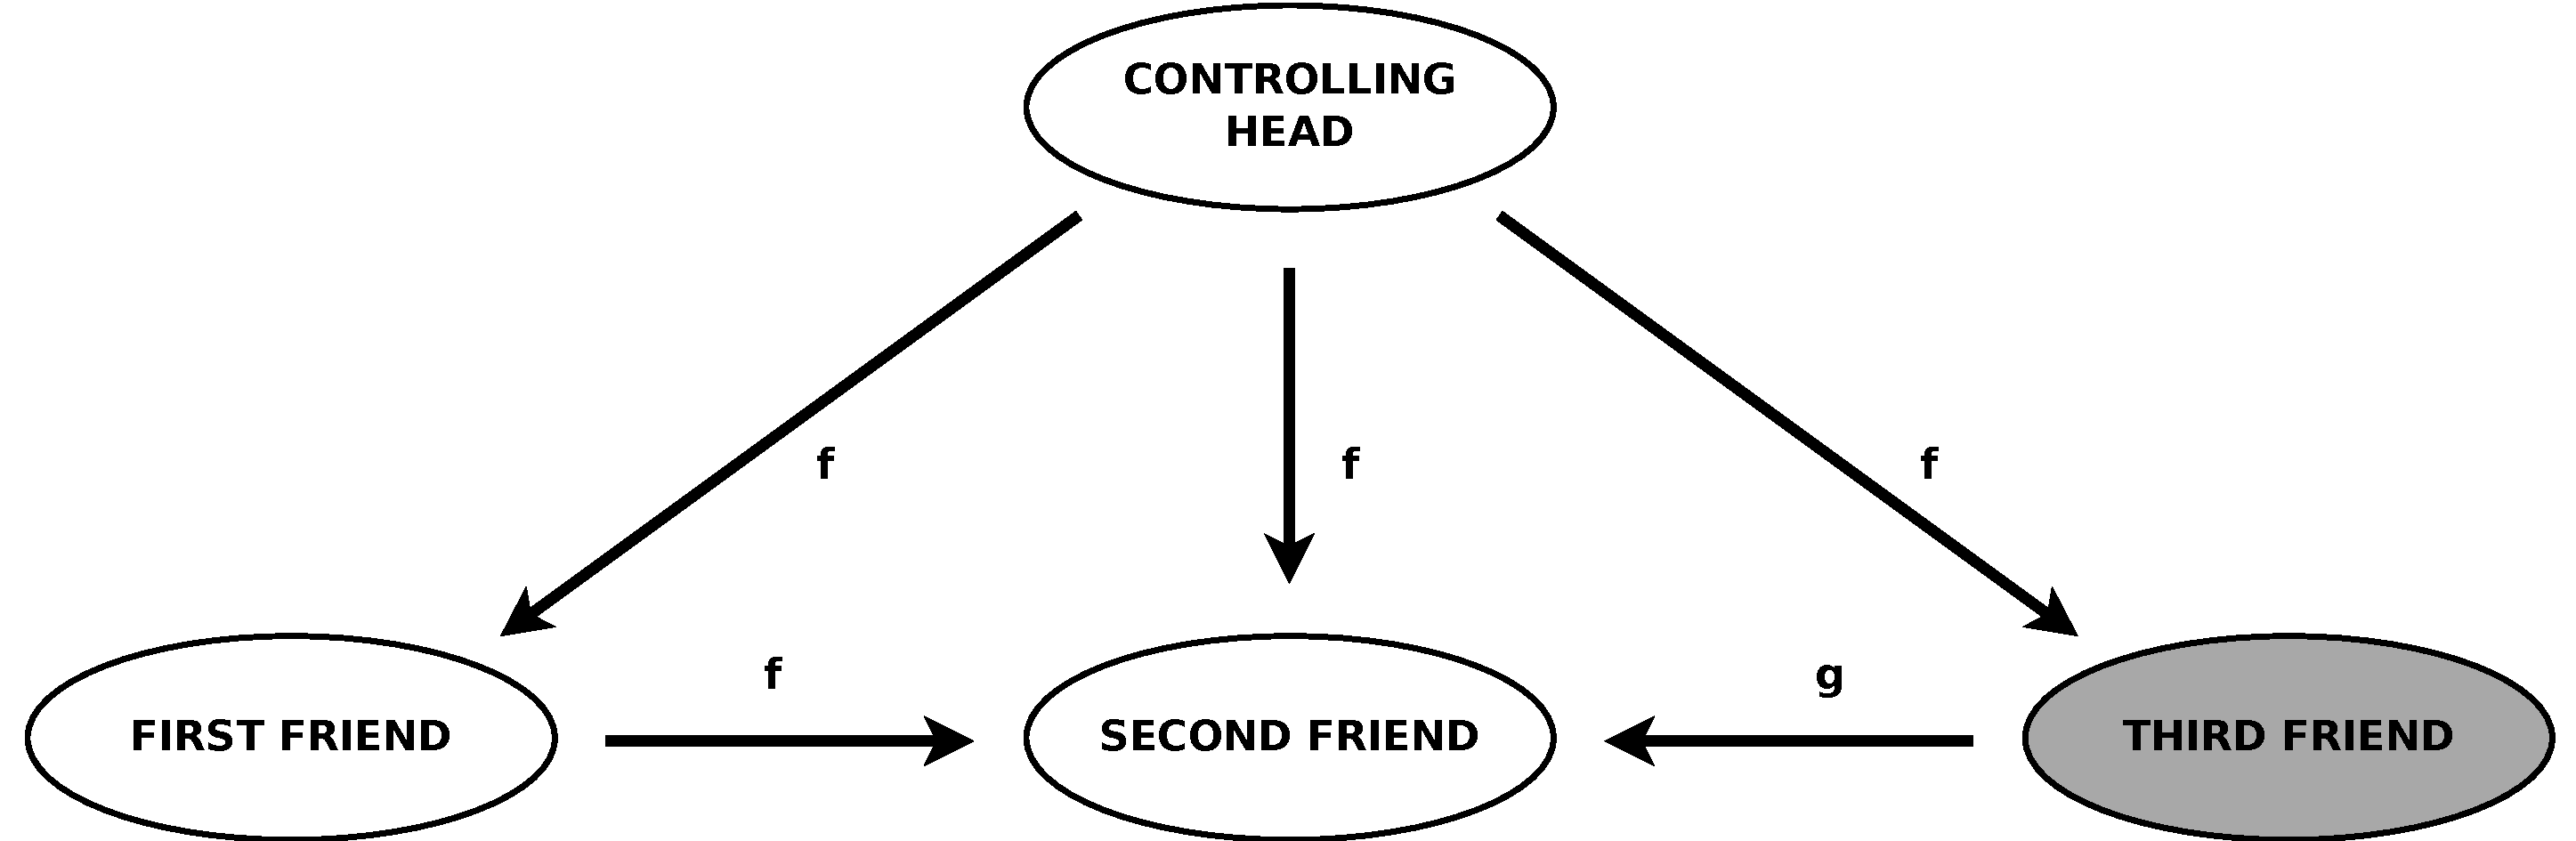
\includegraphics[width=0.75\textwidth]{fig3.pdf}
%	\end{center}
%	\caption{Spoken Words plan, where the third head is a bad guy.}
%	\label{fig:3}
%	%\end{minipage}\end{sideways}
%\end{figure}
%\begin{figure}[h]
%	%\begin{sideways}\begin{minipage}{\textwidth}
%	\begin{center}
%		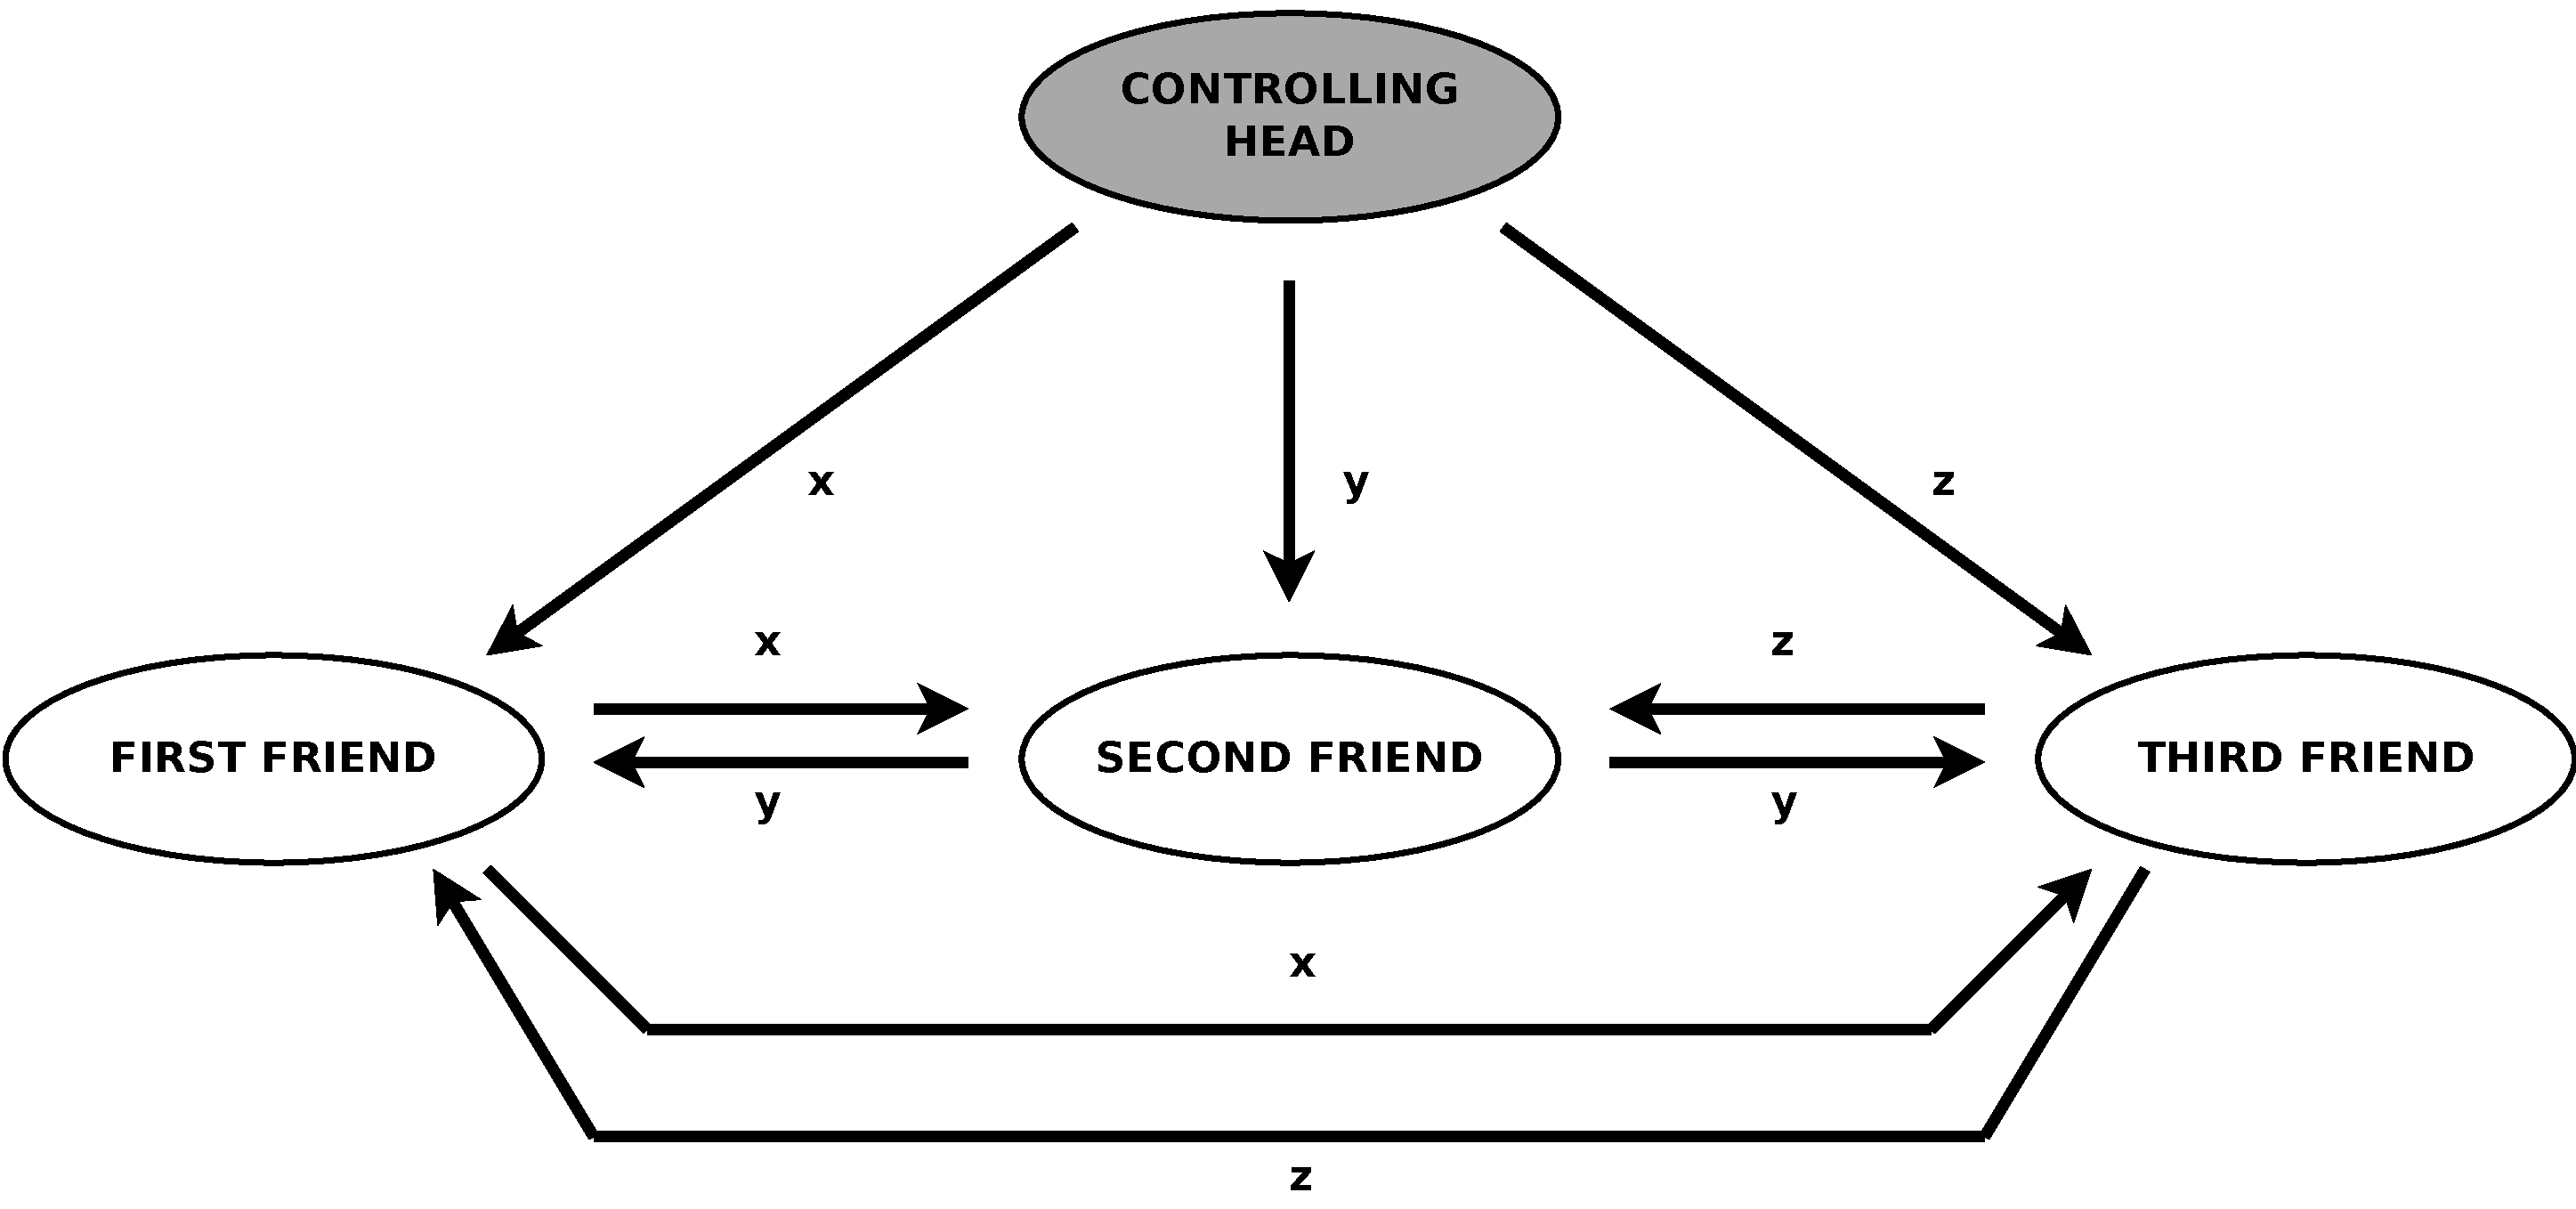
\includegraphics[width=0.75\textwidth]{fig4.pdf}
%	\end{center}
%	\caption{Spoken Words plan, where the controlling head is a bad guy.}
%	\label{fig:4}
%	%\end{minipage}\end{sideways}
%\end{figure}

% TODO: If you rewrite the introduction, readjust this
In step (1), the good-guy controlling head sends an order to all $n - 1$ of their friends. In step (2),
each good-guy friend runs the Spoken Words plan for $m-1$ bad guys with $n-1$ heads. Since we supposed $n$ is bigger than $2k+m$, we know $n-1$ is bigger than $2k+(m-1)$, so we can use the thing we supposed to show that every good-guy friend decides to do what the controlling head told them. Since there are at most $k$ bad guys, and $n-1$ is bigger than $2k+(m-1)$, which in turn is bigger than two times $k$, then more than half of the friend-heads are good guys. So, each good-guy friend decides to do what the controlling head told them in the third step, which makes sure that FA2 happens.
\qed

The following expression says that the Spoken Words plan is a right answer to the \prob.

\begin{mylemma}
For any number of bad guys, the Spoken Words plan makes sure both Friends-Agreeing situations happen if there are more than three times as many people as bad guys.
\end{mylemma}


{\sc Reason That is True.}
We show the reason this is true by the same way of supposing as before. If there are no bad guys, then it is easy to see that the easiest Spoken Words plan makes situations FA1 and FA2 happen. So, we suppose that the expression is true for the Spoken Words plan for $m-1$ bad guys, and show it is true for $m$ bad guys.

We first consider the case in which the controlling head is good. By letting $k$ be the same as $m$ in Expression~\ref{lemma:1},
we see that the Spoken Words plan for $m$ bad guys makes FA2 happen. FA1 follows from FA2 if the controlling head is good, so we need only make sure FA1 happens in the case that the controlling head is a bad guy.

There are at most $m$ bad guys, and the controlling head is one of them, so at most one fewer than $m$ of their friends are also bad guys. Since there are more than three times $m$ people in total, there are more than $3m-1$ friends, and one fewer than three times $m$ is bigger than three times one fewer than $m$. So we can use the thing we supposed to show that the Spoken Words plan for $m-1$ bad guys makes FA1 and FA2 happen.
Because of that, any two good-guy friend-heads decide to do the same thing in the third step of the plan, which makes FA1 happen.
\qed

\section{A plan for when bad guys can't pretend their words came from someone else}
\label{sec:4}

As we saw from the situations in Figures 1 and 2, it is the fact that bad guys can lie that makes the \shortprob~so hard.
The problem becomes easier to find an answer for if we can make sure they don't lie. One way to do this is to let the heads send signed letters to each other. Using computers, there are ways to sign your letters where you use some very big numbers that make it very hard for a bad guy to pretend a signed letter was written by someone else or says something different. We'll suppose the heads use this way of signing letters. So, already supposing A1, A2, and A3, we will also suppose the following: \\
\\
\begin{tabular}{p{0.8em}p{0.8em}p{0.9\textwidth}}
A4 & (a) &
A bad guy can't write a signed letter and pretend that a good guy wrote it, and also can't change a signed
letter that was already written to say something else. \\
& (b) & Anyone can make sure that a signed letter came from the person who signed it.
\end{tabular} \\

Note that we don't suppose anything about letters that a bad guy signed. One important thing this means is that bad guys can write signed letters and pretend they came from other bad guys. So we are even letting bad guys work together instead of acting alone.

Now that we can write signed letters, the thing we said earlier about needing four or more heads in order to be okay with one bad guy is no longer true. In fact, there is an answer for three heads now. We now give an answer where any number of heads are okay with any number of bad guys (though the problem doesn't make any sense if there are fewer than two good guys).

Usually, when signing a letter, you write your name at the bottom of the letter. But since we are using computers and very big numbers for this stronger sort of signing, the thing you write after the letter is numbers, instead of your name. We will call these ``signing-numbers''.

In our answer, the controlling head sends a signed order to each of her friends.
Each friend then adds his or her signing-numbers to that order and sends it to the other friends, who add their signing-numbers to that order and send it to everyone else, and so on.
This means that each head must be given one signed letter and sign it and send it to several other people.
% omitted discussion of what it means to copy and choice(V)

In the following answer, when we say $f:i$, we mean the fact $f$ signed by head number $i$. So, $f:j:i$ means the fact $f$ signed by head $j$, and then that fact-and-signing-numbers signed again by head $i$. We will say Head One is the controlling-head, who gives the orders. In this plan, each head remembers a set $V_i$ which is made of all (not pretended) signed orders he or she has been given so far. (If Head One is a good guy, then this set should never have more than one thing in it.)

Do not confuse $V_i$, the set of orders that a head was given, with the set of words that were said to them. There may be many different words spoken about the same order. \\

{\em Spoken Words Plan for $m$ bad guys.} \\
\\
At the start, each $V_i$ is empty.
\begin{enumerate}
	\item The controlling head signs and sends her order to every friend head.
	\item For each $i$:
	\begin{enumerate}
		\item If head number $i$ is given a letter of the form $f : 1$ from the controlling head and he has not yet heard any order, then
		\begin{enumerate}
			\item he lets $V_i$ become just $\{v\}$;
			\item he sends the signed letter $v: 1 : i$ to every other head.
		\end{enumerate}
		\item If head number $i$ gets a letter of the form $f : 1 :j_1 : \dots : j_k$ and $v$ is not in the set $V_i$, then
		\begin{enumerate}
			\item he adds $v$ to $V_i$;
			\item if $k$ is less than $m$ (the number of bad guys), then he sends the letter $f:1 :j_i1 : \dots :j_k : i$ to every head besides the ones with numbers $j_1$ through $j_k$.
		\end{enumerate}
	\end{enumerate}
	\item For each $i$: When head number $i$ will get no more letters, he or she decides to follow any order in the set $V_i$, or RUN AWAY if the set is empty.
\end{enumerate}

Note that in step (2), the heads ignore any letter that talks about an order already in the set $V_i$.

% omitted: how to decide when no more messages are coming

\begin{figure}[ht]
	\begin{center}
		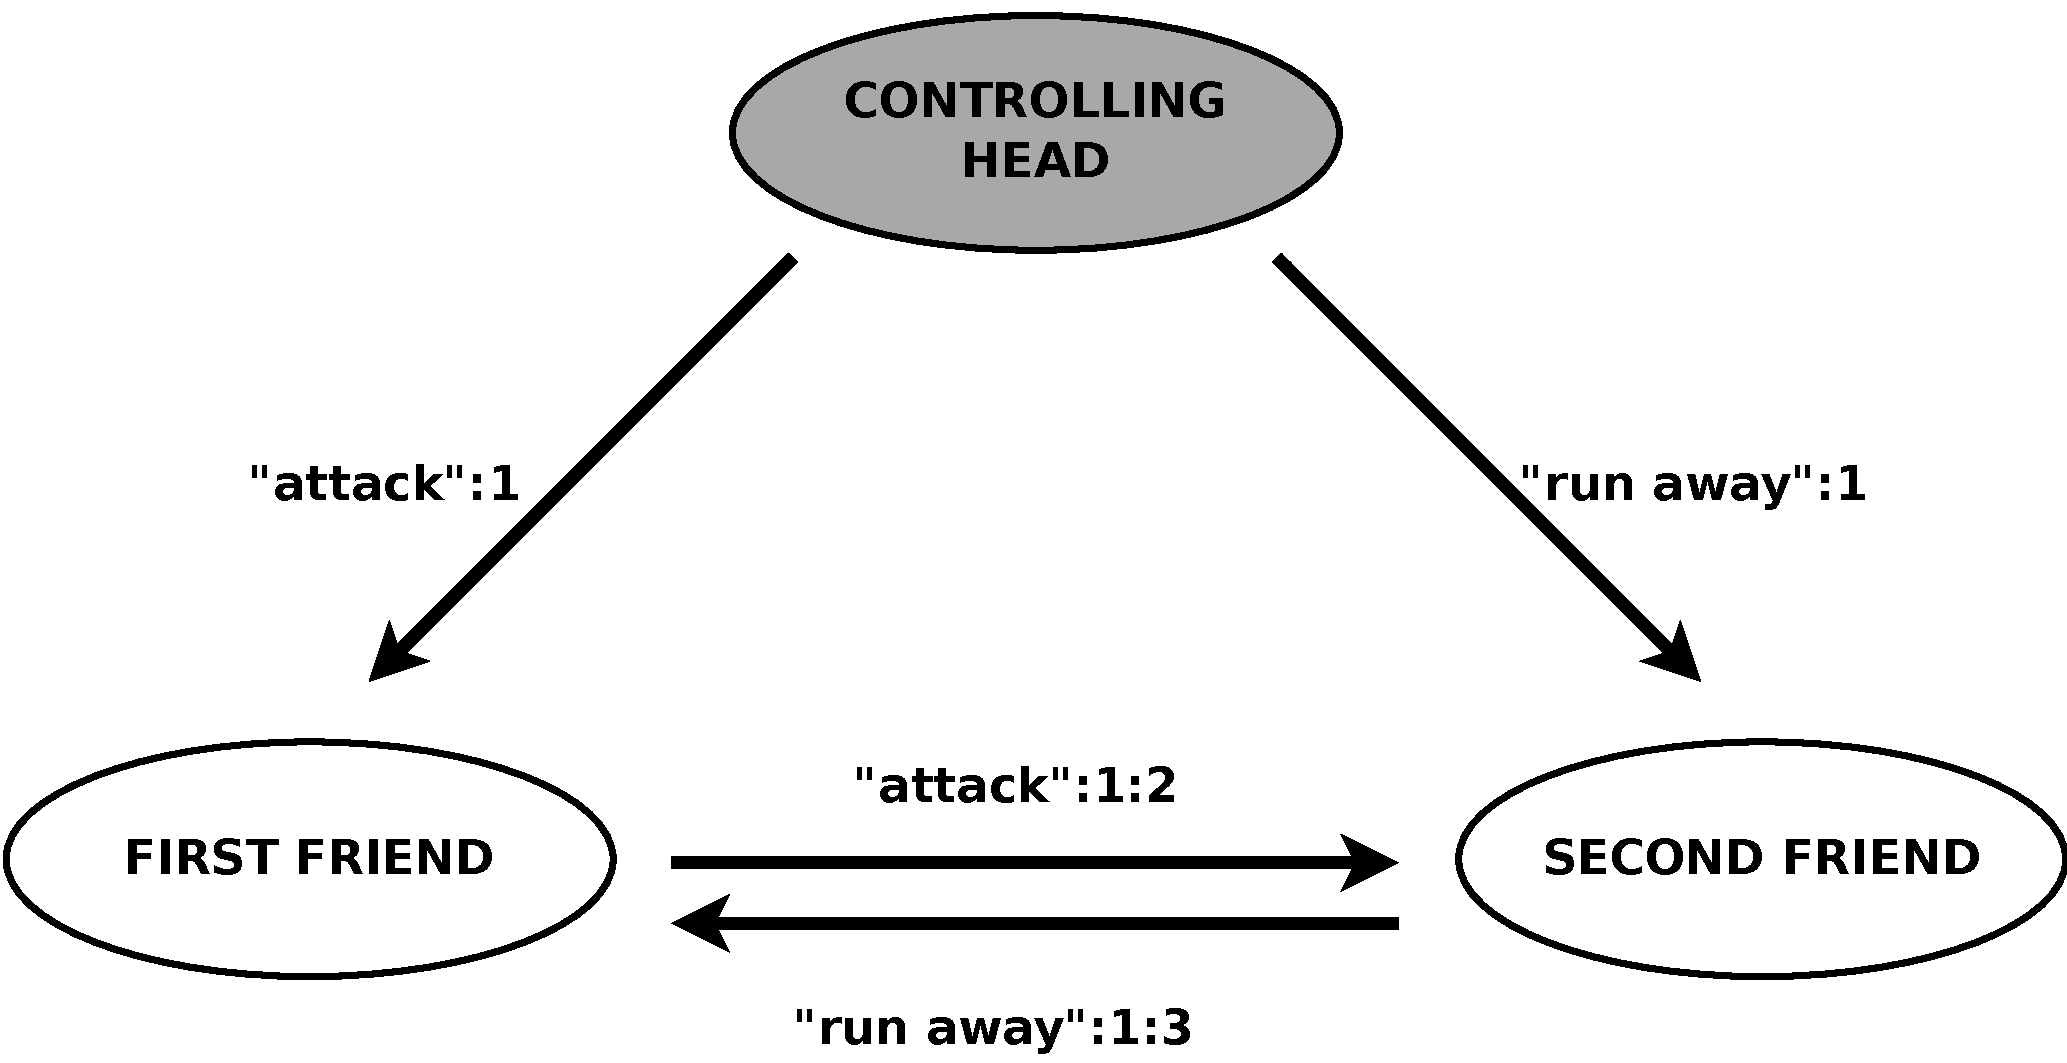
\includegraphics[width=0.7\textwidth]{fig5.pdf}
	\end{center}
	\caption{Signed Letters plan, with the controlling head as a bad guy}
	\label{fig:5}
\end{figure}

Figure~\ref{fig:5} shows the Signed Letters plan for the case of three heads when the controlling head is a bad guy. The controlling head sends an ``attack'' order to one head and a ``run away'' order to another. Both
friend-heads get the same two orders in step (2), so after step (2) $V_2$ and $V_3$ are both \{``attack'', ``run away''\}, and they both decide what to do the same way.
Notice that here, which is not like the situation in Figure~\ref{fig:2}, the friends know that the controlling head is a bad guy because she signed two different orders, and A4 states that only she could have made those signing-numbers.

% omitted: correctness proof

% omitted: missing communication paths

% omitted: \section{Groups of computers that you can trust}

\section{Closing Words}

We have presented several answers to the \prob, in several different situations.
The plans in these answers can take a lot of time to run and can also need a lot of letters to be sent.
Both the Spoken Words plan and the Signed Letters plan might need each order to be sent more than $m$ times, where $m$ is the number of bad guys.

In other words, each head may have to wait for orders that came from the controlling head and were then passed on by $m$ other heads.
Other people who study computers
have shown that this must be true for any answer that can be okay with with $m$ bad guys, so our answers are as good as possible.

The Spoken Words plan and the Signed Letters plan need you to send up to $(n-1)$ times $(n-2)$ times (and so on\dots) times $(n-m-1)$ letters or words. You can make the number of different times you need to send lower by putting letters or words together and sending them at the same time.
It may also be possible to lower how much you actually need to say at all, but we have not studied this enough to be sure.
However, we expect that a large number of letters will still be needed.

Making a group of computers that you can trust even when there might be bad guys that try to confuse you in whatever way they want is a hard problem. It seems like any plan to do this will need to take a lot of time or space.
The only way to make it need less is to start supposing things about the way things might go wrong.
One such way is to suppose that a computer may stop responding but will never respond with something confusing.
However, when you need to trust your computers very very much, you can't suppose that sort of thing, and you need to spend all time and space it takes to find an answer for the \shortprob.

% Bibliography
\section*{PAST THINGS THAT WE BUILT ON}

{\small
\begin{tabular}{p{0.3em}p{0.95\textwidth}}
1.& {\sc Monroe, R.} Up Goer Five. {\em XKCD Computer Funny Pictures,} \url{http://xkcd.com/1133/}, 2013.\\
2.& {\sc Sanderson, T.} The Up-Goer Five Word-Writing Computer Game. \url{http://splasho.com/upgoer5/}, 2013.\\
3.& {\sc Pease, M., Shostak, R., and Lamport, L.} Reaching a Way to Agree Even When There are Faults. {\em J. ACM 27,} 2 (Month Four 1980), 228-234.
\end{tabular}
}

% History dates
\received{Month Four 1980}{Month Ten-and-One 1981}{Month Four 2013}


% \elecappendix
% \section{Analysis of Invalid Trials}

\end{document}
